\documentclass[12pt, twoside]{article}
\usepackage[letterpaper, margin=1in, headsep=0.5in]{geometry}
\usepackage[english]{babel}
\usepackage[utf8]{inputenc}
\usepackage{amsmath}
\usepackage{amsfonts}
\usepackage{amssymb}
\usepackage{tikz}
\usetikzlibrary{quotes, angles}
\usepackage{graphicx}
\usepackage{enumitem}
\usepackage{multicol}
\usepackage{hyperref}

\newif\ifmeta
\metatrue %print standards and topics tags

\title{IB Mathematics}
\author{Chris Huson}
\date{September 2021}

\usepackage{fancyhdr}
\pagestyle{fancy}
\fancyhf{}
\renewcommand{\headrulewidth}{0pt} % disable the underline of the header
\raggedbottom


\fancyhead[LE]{\thepage}
\fancyhead[RO]{\thepage \\ Name: \hspace{4cm} \,\\}
\fancyhead[LO]{BECA / IB Math 03-Quadratic functions\\* 7 January 2022}

\begin{document}

\subsubsection*{3.4 Graphing quadratic functions}
\begin{enumerate}
\item The function $f(x)=-x^{2}+2x+3$ is shown on the graph.
    \begin{enumerate}[itemsep=1.2cm]
      \begin{multicols}{2}
          \item Write down its vertex as an ordered pair.
          \item Write down $f(0)$.
          \item Write down two solutions to $f(x)=0$. 
          \item Hence or otherwise, write $f$ in the form $f(x)=a(x-p)(x-q)$\vspace{3cm}
          \begin{center}
          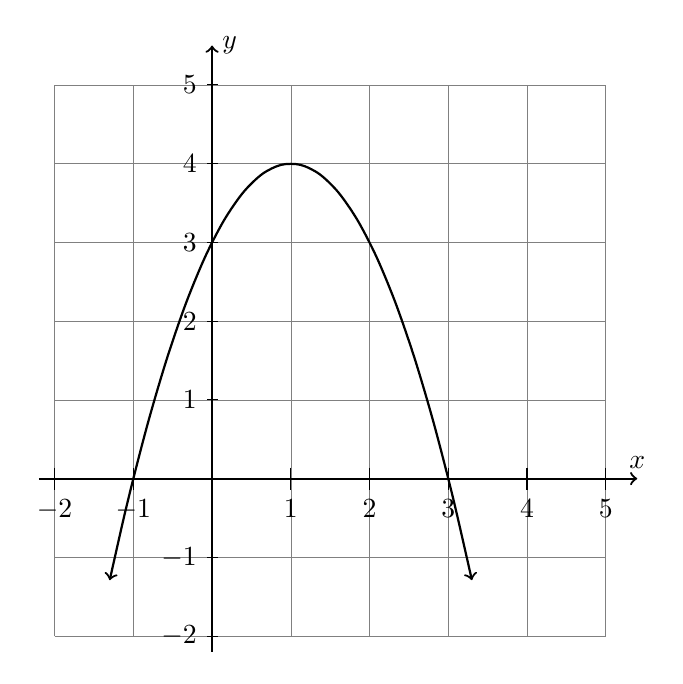
\begin{tikzpicture}[scale=1]
            \draw [help lines] (-2,-2) grid (5,5);
            \draw [thick, ->] (-2.2,0) -- (5.4,0) node [above] {$x$};
            \draw [thick, ->] (0,-2.2)--(0,5.5) node [right] {$y$};
            \foreach \x in {-2,-1, 1,2, ...,5} \draw (\x cm,4pt) -- (\x cm,-4pt) node[below] {$\x$};
            \foreach \y in {-2,...,-1,1,2,..., 5} \draw (2pt,\y cm) -- (-2pt,\y cm) node[left] {$\y$};
            %\fill (-1,0) circle[radius=0.1] node[above left]{$j$};
            %\fill (3,0) circle[radius=0.1] node[above right]{$k$};
            \draw [thick, <->,smooth,samples=20,domain=-1.3:3.3] plot(\x,-\x*\x+2*\x+3);
          \end{tikzpicture}
          \end{center}
        \end{multicols}
    \end{enumerate} \vspace{2cm}
    
\item   Given $f(x)=(x+2)(x-6)$
    \begin{enumerate}[itemsep=0.9cm]
        \begin{multicols}{2}
        \item Sketch the function. Label the vertex as an ordered pair and mark the intercepts with their values.
        \item Expand the function to standard form, $f(x)=ax^2+bx+c \text{ where } a, b, c \;  \epsilon \; \mathbb{R}$. \vspace{3.5cm}
        \begin{center}
            \begin{tikzpicture}
                \draw [thick, ->] (-4,0) -- (+4,0) node [below left] {$x$};
                \draw [thick, ->] (0,-5.5) -- (0,3.5) node [left] {$y$};
            \end{tikzpicture}
            \end{center}
        \end{multicols}
    \end{enumerate}

\newpage
\item Consider the graph given by the equation $y=0.4x^2-2x-8$.
    \begin{enumerate}[itemsep=1cm]
        \item Find the coordinates where the graph crosses the $x$-axis.
        \item Find the coordinates of the intercept with the $y$-axis.
        \item Find the equation of the axis of symmetry of the curve.
        \item Sketch the graph and the axis of symmetry, marking the intercepts and vertex.
    \end{enumerate}
    \begin{center}
    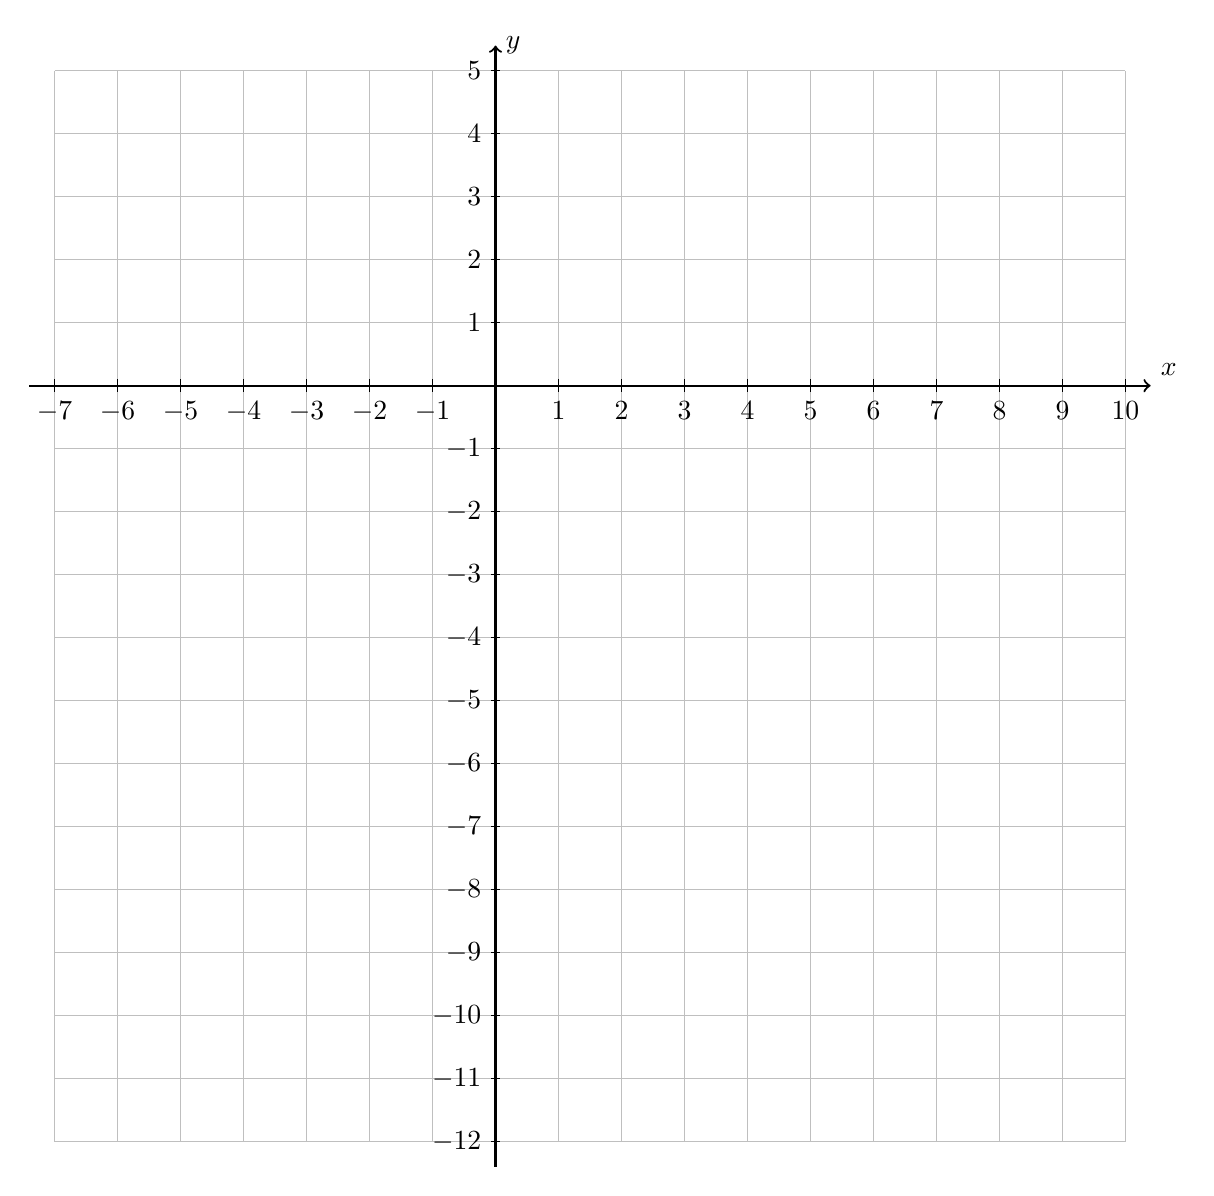
\begin{tikzpicture}[scale=0.8]
        \draw [thin, color=lightgray,, xstep=1.0cm,ystep=1.0cm] (-7,-12) grid (10,5);
        \foreach \x in {-7,...,-1,1,2,...,10}
        \draw (\x cm,3pt) -- (\x cm,-3pt) node[below] {$\x$};
        \foreach \y in {-12,...,-1,1,2,...,5}
        \draw[shift={(0,\y)},color=black] (2pt,0pt) -- (-2pt,0pt) node[left]  {$\y$};
        \draw [thick, ->] (-7.4,0) -- (+10.4,0) node [above right] {$x$};
        \draw [thick, ->] (0,-12.4) -- (0,5.4) node [right] {$y$};
        %\draw [thick, <->,smooth,domain=-3.5:8.5] plot(\x,0.4*\x*\x-2*\x-8);
    \end{tikzpicture}
    \end{center}

\newpage
\item A ball is thrown vertically upwards.\\[0.25cm]
The path of the ball can be modelled by the equation $h(t)=12t-4t^2$ where $h(t)$ is the height of the ball after $t$ seconds.
    \begin{enumerate}
        \item Plot a graph of this equation and hence sketch it below, showing the coordinates of the vertex and axes intercepts.
        \item Find the $t$-intercepts and explain what these values represent. \vspace{2cm}
        \item Find the equation of the axis of symmetry, and state what this tells you in the context of the problem. \vspace{2cm}
    \end{enumerate}
    \begin{center}
    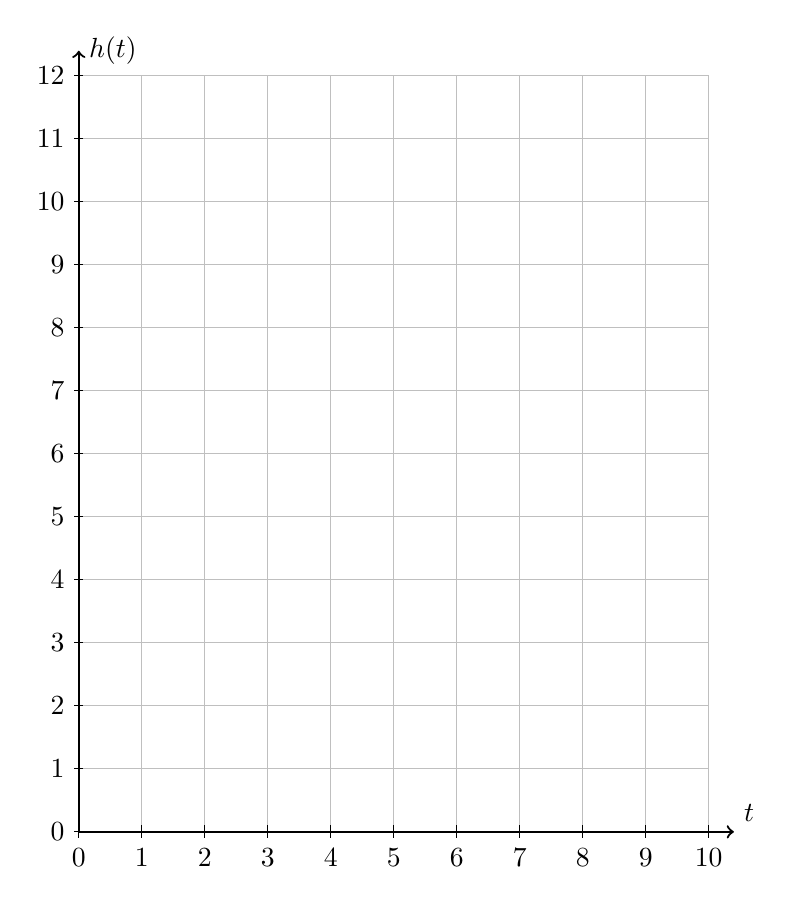
\begin{tikzpicture}[scale=0.8]
        \draw [thin, color=lightgray,, xstep=1.0cm,ystep=1.0cm] (0,0) grid (10,12);
        \foreach \x in {0,1,2,...,10}
        \draw (\x cm,3pt) -- (\x cm,-3pt) node[below] {$\x$};
        \foreach \y in {0,1,2,...,12}
        \draw[shift={(0,\y)},color=black] (2pt,0pt) -- (-2pt,0pt) node[left]  {$\y$};
        \draw [thick, ->] (0,0) -- (+10.4,0) node [above right] {$t$};
        \draw [thick, ->] (0,0) -- (0,12.4) node [right] {$h(t)$};
        %\draw [thick, <->,smooth,domain=-3.5:8.5] plot(\x,0.4*\x*\x-2*\x-8);
    \end{tikzpicture}
    \end{center}
    
\newpage
\item The path of a football can be modeled by the quadratic equation\\[0.25cm]
$h(x)=-0.0125x^2+0.65x-3.45$ \\[0.25cm]
where $h(x)$ is the height of the ball in meters, and $x$ is the horizontal distance of the football in meters.
    \begin{enumerate}
        \item Sketch the graph below, labeling the coordinates of the vertex and axes intercepts.
        \item Explain what the vertex represents in context. How high was the ball kicked?\vspace{2cm}
        \item Find the $x$-intercepts and explain what these values represent. How far was the ball kicked?\vspace{2cm}
    \end{enumerate}
    \begin{center}
    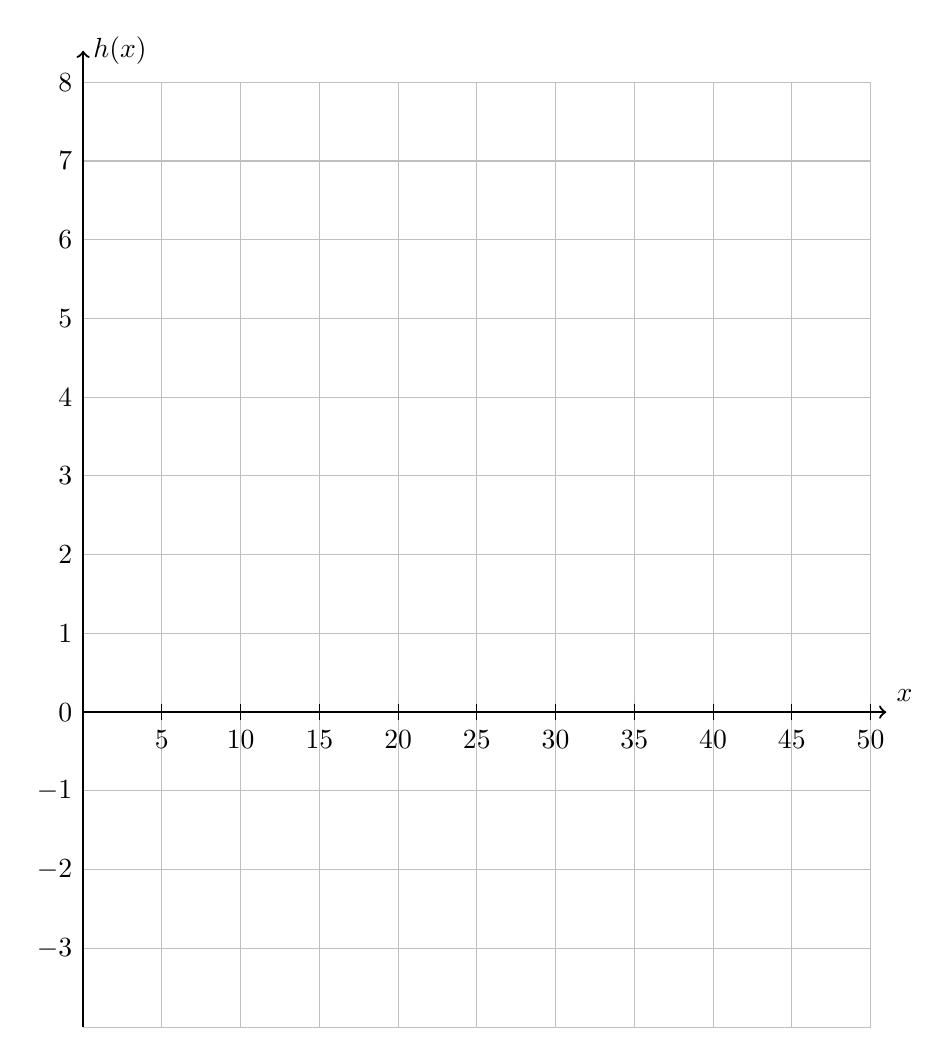
\begin{tikzpicture}[xscale=0.2]
        \draw [thin, color=lightgray,, xstep=5.0cm,ystep=1.0cm] (0,-4) grid (50,8);
        \foreach \x in {5,10,...,50}
        \draw (\x cm,3pt) -- (\x cm,-3pt) node[below] {$\x$};
        \foreach \y in {-3,-2,-1,0,1,2,...,8}
        \draw[shift={(0,\y)},color=black] (2pt,0pt) -- (-2pt,0pt) node[left]  {$\y$};
        \draw [thick, ->] (0,0) -- (+51,0) node [above right] {$x$};
        \draw [thick, ->] (0,-4) -- (0,8.4) node [right] {$h(x)$};
        %\draw [thick, <->,smooth,domain=0:50] plot(\x,-0.0125*\x*\x+0.65*\x-3.45);
    \end{tikzpicture}
    \end{center}

\end{enumerate}
\end{document}